% Copied from my thesis
\section{Information theory}
In the previous section we discussed how a physical perspective on statistics naturally leads to concepts like entropy and algorithms for exploring configuration spaces. In this section we discuss an information theoretic perspective which abstractly considers the sequence of coin flips as a message to be transmitted, allowing us to reckon with the inherent complexity of the data observed in a general sense. 

Central to information theory is a thought experiment aiming to \emph{encode} a message as efficiently as possible. Suppose we would like to transmit to another party the results of our earlier experiment of 10 coin flips as the message "HHTTHTTHTT." Suppose further that we are restricted in this communication to use a~\emph{binary channel} which can only send a binary sequence of 0's and 1's of our choosing. We would then like the receiver on the other side of the channel to be able to decode our binary transmission back into our original message. 

Just as we represented the sequence as a physical state vector in the last section, we may now encode these coin flips as the binary string "1100100100" where the digit "1" represents heads and "0" represents tails. This correspondence between meanings and binary strings is known as a \emph{codebook}. So long as we and the receiver agree on the nature of the encoding, the receiver can use the codebook to decode the binary string back into the original message of outcomes. To determine the efficiency of our transmission we measure the length of our binary string in \emph{bits}. In this case our encoding used 10 digits (bits) to transmit the message, one for each flip. A schematic of this encoding framework is given in Figure~\ref{fig:coin-flip-perspectives}c.

This association of digits to outcomes is quite a natural encoding of two-sided coin flips. In a more general setting, however, we will need to be more creative in our transmission. Suppose we would like to send the message "ELEVENELVES" as a binary string. Since this string contains 5 distinct characters, we can no longer encode the message by assigning each character its own binary digit. For lack of digits we must assign some characters to a \emph{codeword} of multiple binary digits. If we are not careful, however, this can render our message ambiguous. If we assign "E" to the codeword "0" and "L" to the codeword "00," the binary message "00" could decode into either "EE" or "L." 

To avoid this polysemy, we can ensure that our transmission is uniquely decodable by using a \emph{prefix-free} (or "instantaneous") code. If no codeword in our codebook is a prefix of another codeword, as the receiver reads the message from left to right the divisions between the codewords will always be clear. Our earlier example was not prefix-free as the codeword "0" is a prefix of the codeword "00," leading to the double meaning. 

Any such prefix-free binary code can be usefully represented as a binary tree whose leaves each correspond to a character (or "symbol") being transmitted. The codeword associated to each symbol is then represented by the path from the root of the tree down to that symbol. Figure~\ref{fig:encoding-examples}a shows an example of such a tree used to encode the five characters. Following the tree paths this "balanced" encoding represents the characters \{"E",~"L",~"V",~"N",~"S"\} with the codewords \{"00",~"01",~"10",~"110",~"111"\} respectively. With this codebook we can then encode the phrase "ELEVENELVES" into pictured binary string of length 24 bits and ensure that it uniquely decodes back into our desired dispatch.

\begin{figure}
    \centering
    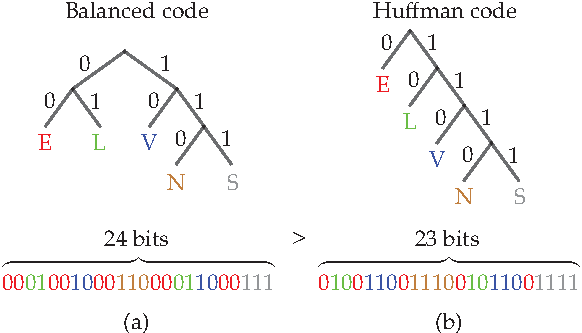
\includegraphics{max_dissertation//chapters//figures//chp1/encoding-examples.pdf}
    \caption{Examples of an (a) balanced code and (b) optimized Huffman code to convert the phrase "ELEVENELVES" into a binary string. The string associated to each letter is denoted by the path from the top of the tree down to the appropriate node. The Huffman code is able to produce a shorter overall message than the balanced code by representing the common letter "E" with a short string "0" despite representing the uncommon letters "N" and "S" with longer strings.}
    \label{fig:encoding-examples}
\end{figure}

Now, a key goal of information theory is not only to successfully transmit a message but also to do so using as few bits as possible. This objective can be seen as a formalization of Occam's razor, the scientific principle that favors the simplest possible answer to a question. In this analogy, transmitting our binary string effectively "explains" to the receiver the data we have observed, making a shorter transmission a more succinct explanation. If we understand predictable patterns in our observations, we can exploit them to construct a more efficient encodings. There is a fundamental duality between \emph{compression} and modeling, as in this context, to compress is to understand. 

In this spirit we can look for patterns in our message to try and come up with a clever way to shorten our encoding. The phrase "ELEVENELVES" has a rather lopsided distribution of characters at 5 E's, 2 L's, 2 V's, 1 N, and 1 S. Some of our codewords are therefore being used in the transmission much more frequently than others. If symbol~$r = 1,...,q$ of the~$q$ symbols appears~$n_r$ times in our message as a codeword of length~$\ell_r$, the total message length is \begin{align}
    \sum_{r=1}^q n_r \ell_r. \label{eq:message-length}
\end{align}
To shorten the overall message we would therefore like the codewords to be as short as possible and to prioritize shortening frequently occurring symbols. In our original encoding the symbol "E" is transmitted with the codeword "00" at a cost of two bits apiece. Since "E" appears so frequently in the message it may be wise to instead represent it with a shorter codeword like "0" and save 5 bits in our total transmission. 

Yet this choice has a cost. If we assign "0" to represent "E" none of the other four characters can be represented with a codeword that begins with a "1" or else the code would no longer be prefix-free. When shortening one codeword we must necessarily lengthen other codewords. This tradeoff is the content of \emph{Kraft's inequality}, which states that the codeword lengths of any prefix-free code must satisfy \begin{align}
    \sum_{r=1}^q 2^{-\ell_r} \leq 1, \label{eq:krafts-inequality}
\end{align}
considering the fraction of the binary tree each codeword occupies. Given the frequencies~$n_r$ at which each symbol appears, we would like to select codeword lengths that minimize the total message length Eq.~\eqref{eq:message-length} subject to the prefix-free constraint Eq.~\eqref{eq:krafts-inequality}.

\emph{Huffman codes} strike this balance and provably minimize the message length by assigning short codewords to frequent symbols while saturating Kraft's inequality. Figure~\ref{fig:encoding-examples}b contains an example of a Huffman code for our application. The code shortens the codeword for "E" from 2 to 1 bit while lengthening the codewords for "N" and "S" from 3 to 4 bits. Since "E" appears much more frequently than "N" and "S," this change shortens the overall message from 24 to 23 bits. By adapting the encoding to the nature of the data, the Huffman code achieves a more parsimonious representation of the message.

More generally given a frequency distribution~$\{n_r\}$ of symbols one can always construct a Huffman code with a simple recursive algorithm. The resulting optimal codeword lengths~$\{\ell_r\}$ follow a predictable pattern. If a symbol appears at a fraction~$p_r = \frac{n_r}{n}$ among the $n$ total symbols, the length of its associated codeword satisfies \begin{align}
      -\log_2(p_r) \leq \ell_r < -\log_2(p_r) + 1.
\end{align} 
Frequent symbols with high probability~$p_r$ are thus assigned small codewords as~$-\log_2(p_r)$ is small while infrequent symbols use longer codewords. In our "ELEVENELVES" example, the character "E" appears with probability $p = 5/11$, and is so assigned a string of length~$1 \approx \log_2(11/5)$ while the character "S" appears at the ratio~$1/11$ and is encoded using~$4 \approx \log_2(11)$ bits. 

In most contexts we consider, symbol probabilities are small and codeword lengths are long. In this regime we can approximate lengths as~$\ell_r = -\log_2(p_r)$, which would in fact be the optimal choices if the lengths could be non-integral numbers of bits. Using these optimal codeword lengths, the minimum message length per symbol is \begin{align}
    S[\{p_r\}] = \frac{1}{n} \sum_{r=1}^q n_r \ell_r = -\sum_{r=1}^q p_r \log_2 p_r, \label{eq:shannon-entropy-discrete}
\end{align}
known as the \emph{Shannon entropy} (or simply "entropy") of the distribution~$\{p_r\}$. For continuous distributions~$P(\vec{x})$ this entropy generalizes to \begin{align}
S[P] = -\int P(\vec{x}) \log_2 P(\vec{x}) d\vec{x}. \label{eq:shannon-entropy-continuous}
\end{align} 
By providing an information theoretic lower bound on transmission, the Shannon entropy captures the inherent information content of a probability distribution that no amount of clever encoding tricks can overcome. 

We can make contact between this information-theoretic entropy and the physical entropy described in Section~\ref{app:statistical-physics}. There the microcanonical ensemble is the uniform distribution~$P(\vec{s}) = \frac{1}{\Omega}$ over all possible configurations that conserve the total energy. The Shannon entropy Eq.~\eqref{eq:shannon-entropy-discrete} then agrees which the microcanonical entropy $S = \log \Omega$ of Eq.~\eqref{eq:S-log-Omega}. In this perspective the additional information cost reflects the added information cost required to specify one of many possible configurations. 

We also note that among all possible distributions~$\{p_r\}$ on~$q$ objects, the uniform distribution has the highest possible entropy since by the convexity of the logarithm \begin{align}
    S[\{p_r\}] = -\sum_{r=1}^q p_r \log p_r \leq -\sum_{r=1}^q \frac{1}{q} \log \left(\frac{1}{q}\right) = \log q.
\end{align}
Therefore the microcanonical ensemble can be therefore be viewed as a \emph{maximum-entropy} distribution over possible configurations. Since the entropy is maximized, the distribution is structure-less, we fundamentally assume that at the level of microstates there are no distinguishing patterns to leverage in equilibrium to craft a more efficient representation, to reduce the entropy. 

The canonical ensemble~$P(\vec{s}) \propto e^{-\beta H(\vec{s})}$ can likewise be motivated as a maximum entropy distribution with a given average energy, which determines the choice of~$\beta$. When designing priors for Bayesian inference, we will frequently appeal to this minimally assumptive principle and choose maximum-entropy priors subject to certain constraints we expect the system to provide. For example, a Gaussian distribution can be motivated as the maximum entropy distribution of a real random variable of a fixed mean and variance. 

Returning to encodings, to obtain the entropy we had considered the total message length of a Huffman code optimized to send that particular message. However in many contexts we do not \textit{a priori} know what distribution of symbols to expect. If before the transmission we believe that the symbols will be distributed with probabilities~$\{q_r\}$ we should optimize our Huffman code accordingly to have code lengths~$\ell_r = -\log q_r$. If in reality, however, the symbols we must transmit have probabilities~$\{p_r\}$ the average code length will be \begin{align}
    \sum_r p_r (-\log q_r).
\end{align}
Had we used code lengths~$-\log p_r$ attuned to the true distribution, this would give the entropy lower bound. But since the our encoding is \emph{misspecified} it will require a larger number of bits to transmit. The shortfall between the two, the extra cost we incur, is known as the \emph{Kullback-Leibler (KL) divergence} \begin{align}
    D_{\text{KL}}(\{p_r\}||\{q_r\}) &= \left(\sum_{k=1}^q p_r (-\log q_r) \right) - \left(\sum_{k=1}^q p_r (-\log p_r) \right) \nonumber \\
    &= \sum_{k=1}^q p_r \log \frac{p_r}{q_r} \geq 0.
\end{align}

This story repeats when modeling data. Given a model with distribution~$Q(\vec{x})$ we can write the Huffman code length (or \emph{description length}) of an observation~$\vec{x}$ as \begin{align}
    H(\vec{x}) = -\log Q(\vec{x}),
\end{align} 
which we can compare to the Hamiltonian in Eq.~\eqref{eq:energy-posterior-relation}. If we use this model encoding on a stream of observations whose true distribution is~$P(\vec{x})$, the average description length decomposes as \begin{align}
    \sum_{\vec{x}} P(\vec{x}) H(\vec{x}) &= -\sum_{\vec{x}} P(\vec{x})\log P(\vec{x}) + \sum_{\vec{x}} P(\vec{x})\log \frac{P(\vec{x})}{Q(\vec{x})} \nonumber \\
    &= \underbrace{S[P]}_{\text{entropy}} +  \underbrace{D_{\text{KL}}(P||Q)}_{\text{cross-entropy}}
\end{align}
into the inherent entropy of the data and the \emph{cross-entropy} cost of our model misspecification. As we model the random process this average description length can never fall below the entropic lower bound, however any description length above this point is evidence of the failure of our model. Although measuring this average description length of a model is a simple matter, deducing what fraction of it is due to the entropy or the cross-entropy is a hard problem. When comparing the average description lengths of two models on the same stream of data, however, we can confidently attribute their difference to a difference in the cross-entropies and prefer the model with the smaller average description length. This motivates the \emph{minimum description length} (MDL) principle, which prefers models whose corresponding encodings across realistic data sets are as small as possible. 

As an application, suppose that we would like to select the appropriate value of a parameter~$\vec{\theta}$ for a model~$P(\vec{x}|\vec{\theta})$. For each choice of parameter the corresponding model description length is simply the minus log-likelihood~$H(\vec{x}|\vec{\theta}) = -\log P(\vec{x}|\vec{\theta})$. Choosing the model that minimizes the description length therefore amounts to finding the maximum-likelihood estimate of the parameter as \begin{align}
    \text{argmin}_{\vec{\theta}} H(\vec{x}|\vec{\theta}) = \text{argmax}_{\vec{\theta}} P(\vec{x}|\vec{\theta}).
\end{align}

As discussed in Section~\ref{app:statistical-inference}, however, this maximum likelihood estimation is prone to overfitting. This approach is also problematic from an information-theoretic perspective. In our optimization of the transmission we have neglected the cost of transmitting the parameter~$\vec{\theta}$ itself. In the Bayesian context this parameter will be distributed according to a prior~$P(\vec{\theta})$ that corresponds to its own encoding \begin{align}
    H(\vec{\theta}) = -\log P(\vec{\theta}). \label{eq:H-log-P-information}
\end{align}
If we consider the total information cost of this now two stage process of first transmitting the parameter~$\vec{\theta}$ and then the data~$\vec{x}$ given that parameter, we recover Bayesian \emph{maximum a posteriori} (MAP) estimation \begin{align}
    \text{argmin}_{\vec{\theta}} \left[H(\vec{x}|\vec{\theta}) + H(\vec{\theta})\right] &= \text{argmax}_{\vec{\theta}} P(\vec{x}|\vec{\theta})P(\vec{\theta})  \nonumber \\
    &= \text{argmax}_{\vec{\theta}} P(\vec{\theta}|\vec{x}). \label{eq:MAP-information}
\end{align}

As seen earlier, the maximum likelihood and MAP estimates of a parameter often differ considerably, particularly when a relatively small amount of data is available. In Section~\ref{sec:reduced-mutual-information-paper} on the applications of information theory to network science we will again encounter situations where neglecting certain terms of the transmission process leads to wildly different results.

After the two stage transmission process of Eq~\eqref{eq:MAP-information} we transmit to the receiver both the data of interest~$\vec{x}$ and the best-fit parameter~$\vec{\theta}$ used. When assessing model performance, however, the parameter is often redundant to the data. We can instead holistically evaluate model performance using the Bayesian evidence, the probability that a model generates a particular data~$\vec{x}$ summed over all possible parameters \begin{align}
    P(\vec{x}) = \int P(\vec{x}|\vec{\theta})P(\vec{\theta}).
\end{align} 
The description length of the integrated model is then \begin{align}
    H(\vec{x}) = -\log P(\vec{x}).
\end{align}
Therefore we can motivate model selection on the basis of the Bayesian evidence, as with Bayes factors, as choosing the model that when integrated more efficiently compresses the data.

By interpreting models as encodings of data we can motivate many of the inference and model selection principles. These connections highlight the duality between the compression and modeling of a data set.

To this point, we have considered the Shannon entropy of \emph{probability distributions}. However, much of this thesis focuses on a subtly different notion of the complexity of \emph{objects}. Shannon entropy quantifies the complexity of a probability distribution without regard to the specific objects within that distribution. For instance, suppose that we want to transmit one of two messages: the full text of \textit{Dune} by Frank Hebert or \textit{It} by Stephen King. While each book's content is undoubtedly "complex," our current framework would allow us to "transmit" them with minimal information cost. If we define an encoding where "0" represents the text of \textit{Dune} and "1" stands for \textit{It}, we could send a single "0" to transmit the entirety of \textit{Dune}. This setup might suggest that the inherent information cost of \textit{Dune}'s content is just one bit, which is clearly an unreasonable conclusion.

The problem is that we have overlooked the information cost required to establish the codebooks. If the receiver is unaware of our coding scheme, we must first communicate the full text that each binary digit corresponds to before our transmission. Once this scheme is established, we can indeed send our choice of book with a single bit repeatedly at low cost. However, the initial information cost of creating the codebook is much higher. Shannon entropy measures the information needed to transmit objects drawn from a probability distribution, not the complexity of the objects themselves.

To approach the information content of an object, we should instead turn to the \emph{Kolmogorov complexity}. Certain objects and outcomes appear to be inherently more complicated than others. For example a sequence of coin flips "HHHHHHHHHH" is easy to describe as "10 heads in a row." Even if the sequence was 1000 heads, the outcome would not be much more complex to describe. On the other hand, the pattern of coin flips "HHTTHTTHTT" we observed appears to be more complicated to describe. However, even in this case the coin flips we observed are simply the first 10 digits of~$\pi = 11.00100100..._2$ in binary: a concise, if unusual, explanation. Yet if we are presented with a truly "random" string of coin flips, there is little hope for such an efficient description of the outcomes. The Kolmogorov complexity is meant to capture the difference between these settings and fundamentally measure how structured a given data set is. 

Roughly speaking, the Kolmogorov complexity~$K(\vec{x})$ can be understood as the length of the shortest computer program that would output the object (typically string) in question. In our earlier examples, this program might be "output 10 heads" or "first 10 digits of $\pi_2$" in pseudocode. In our earlier example of books, the full texts may be compressed with a technique like the Lempel-Ziv-Welch algorithm used in the \verb|.gif| file format. The "program" in this case would consist of a description of the LZW algorithm, followed by the compressed file. The total program size, and so complexity will still be fairly large as some fraction of the original length of the book, but is much greater than the single bit we had used to transmit it in a probabilistic sense. 

The "computer program\footnote{More formally a universal Turing machine.}" in the definition of the Kolmogorov complexity is vague enough to accommodate any possible valid encoding or explanation of a string. With this immense flexibility, however, comes the inability to conclusively compute the measure. Although any program that successfully outputs~$\vec{x}$ provides an upper bound on its complexity, it is only possible to show that~$K(\vec{x})$ is above some value~$n$ by checking all possible problems of length less than or equal to~$n$. 

Note that a model~$M$ can also be interpreted as a computer program, where now the instructions are to specify the model, which then defines a distribution over all possible data sets according to the Bayesian evidence, which can then be used to define a Huffman encoding of the data of length~$H_M(\vec{x})$, the description length. Although we neglect the constant overhead associated with describing both the model and this framework, we may then roughly say that an encoding of length~$H_M(\vec{x})$ is possible for the data~$\vec{x}$. 

In practice in this thesis we will look to make approximations of these inherent complexities by minimizing over candidate models with competing description lengths~$H_M(\vec{x})$ of the same data, so that if we have many possible models~$M \in \mathcal{M}$, we roughly consider the information cost \begin{align}
    K(\vec{x}) \sim \text{min}_{M \in \mathcal{M}} H_{M}(\vec{x}).
\end{align}
Of course in this pursuit we cannot consider models too finely attuned to a particular data set, although for our purposes we considering rather generic simple models. We can only hope to ever approximate the Kolmogorov complexity in this sense, although as we find models with shorter distribution length we can (roughly) obtain tighter upper bounds on the truth.

Reveal that the initial random sequence of trials that we observed is the first 10 digits of~$\pi = 11.00100100..._2$ in binary, and that this is then a perfect, concise explanation of the observations but one that we could not find due to our (natural) assumption of independence of the coin flips.

We cannot find the perfect encoding, nor the perfect model but can strive for better understanding within this framework.  With this caveat in mind, we can create models that attempt to explain the nature of the many network data sets that we had considered.